\documentclass[a4paper]{article}

\usepackage[toc,page]{appendix}

\usepackage[spanish]{babel}
\usepackage[utf8]{inputenc}
\usepackage{amsmath}
\usepackage{graphicx}
\usepackage{fancyhdr}
\usepackage{amsmath}
\usepackage[colorinlistoftodos]{todonotes}
\usepackage{xcolor}
\usepackage{minted}
\usepackage[font=small,labelfont=bf]{caption}
\usepackage{enumitem}

\usepackage{hyperref}

\hypersetup{
    colorlinks,
    citecolor=blue,
    filecolor=blue,
    linkcolor=blue,
    urlcolor=blue
}

\newcommand*{\tabulardef}[3]{
  \begin{tabular}[t]{@{}lp{\dimexpr\linewidth-#1}@{}}
    #2&#3
\end{tabular}}

\usepackage{geometry}
\geometry{a4paper}

\begin{document}
\begin{figure}
\centering
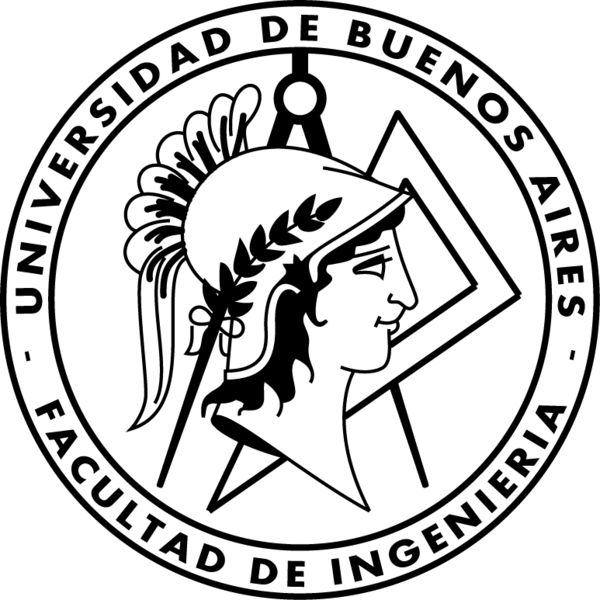
\includegraphics[scale=1]{./img/logo-facu}
\end{figure}

\title{\large\textsc{66.20 - Organización De Computadores}\\
\large Trabajo Práctico 3 - Data Path}

\author{
Andrew Parlane \\
}

\maketitle

\newpage

\tableofcontents

\listoffigures

\newpage

\section{Introducción}

El objetivo de este trabajo se base en familiarizarse con la microarquitectura y la arquitectura de conjuntos de instrucciones de un CPU MIPS. Para simular el data path se usó el programa \textit{DrMIPS}.

\section{Implementación}

El programa \textit{DrMIPS} usa dos archivos de \textit{JSON} para especificar el conjunto de instrucciones \textit{(.set)} y el data path \textit{(.cpu)}. Comencé con una microarquitectura monociclo y una de pipeline, y tuve que implementar las siguientes instrucciones:
\begin{itemize}[noitemsep]
\item J - para la microarquitectura pipeline.
\item JR - para los dos CPUs.
\item JALR - para los dos CPUs.
\end{itemize}

\subsection{J para pipeline.cpu}

La instrucción J (para Jump) tiene opcode 2 (6 bits) y los otros 26 bits están el target. El resultado es: $PC = ((PC\, +\, 4)\, \&\, 0xF0000000)\, |\, (target << 2)$

Al principio intenté implementar el data path para ese instrucción en la etapa de \textit{IF}. Desafortunadamente DrMIPS no tiene forma fácil para decodificar una instrucción sin usar un bloque de control, y solo puede haber un bloque de control en el data path. Así tuve que implementarle en la etapa de \textit{ID} y introducir un ciclo de stall.

Figura \ref{fig:j_pipeline} muestra mi implementación. Hay un distribuidor para obtener los 4 bits más altos de PC+4, y un concatenador para juntarle con el target, desplazado a la izquierda dos bits. Hay un MUX para elegir entre ese y \textit{PC+4}. El mux es controlado por la señal \textit{jump} que viene del unidad de control. Finalmente se introduce un ciclo de stall en IF/ID si hay un branch o un salto.

\begin{figure}[h]
\centering
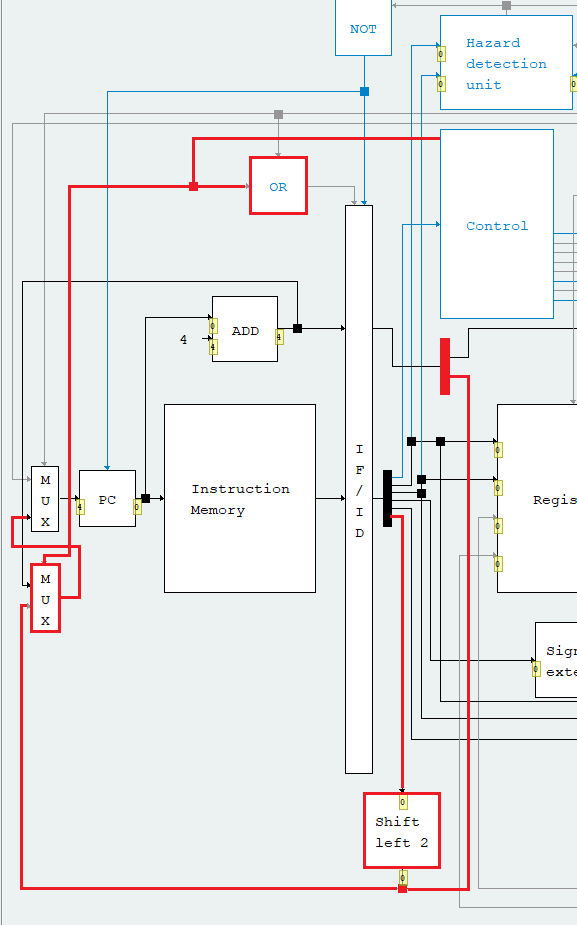
\includegraphics[scale=.5]{./img/j_pipeline.png}
\captionof{figure}{Implementación de la instrución J en la microarquitectura pipeline.cpu }
\label{fig:j_pipeline}
\end{figure}

\subsection{JR para unicycle.cpu}

La instrucción JR (para Jump Register) tiene opcode 0 y es tipo \textit{R}, con Rt, Rd y SHAMT en ceros, y func 8. El resultado es: PC = Rs.

El desafío principal para ese instrucción estuvo cómo decodificar el función. No se puede hacer lo con el unidad de control normal, hay que usar el unidad de control del ALU. Figura \ref{fig:jr_unicycle} muestra mi implementación. Reemplacé los dos muxes que eligieron el nuevo PC, por uno con cuatro entradas. Se elija cual a usar con dos bits concatinados. El bit más alto es "Jump o JumpReg" y el bit más bajo es "Branch o JumpReg".

El unidad de control escribe un uno a la señal RegWrite cuando hay un instrucción con opcode 0. Ese significa que el resultado de la operación del ALU es escrito al registro especificado en Rd. Normalmente esto será un problema porque la instrucción JR no debería cambiar los valores de los registros. Pero para Rd es cero, así escribe al registro R0 que siempre es cero.

\begin{figure}[h]
\centering
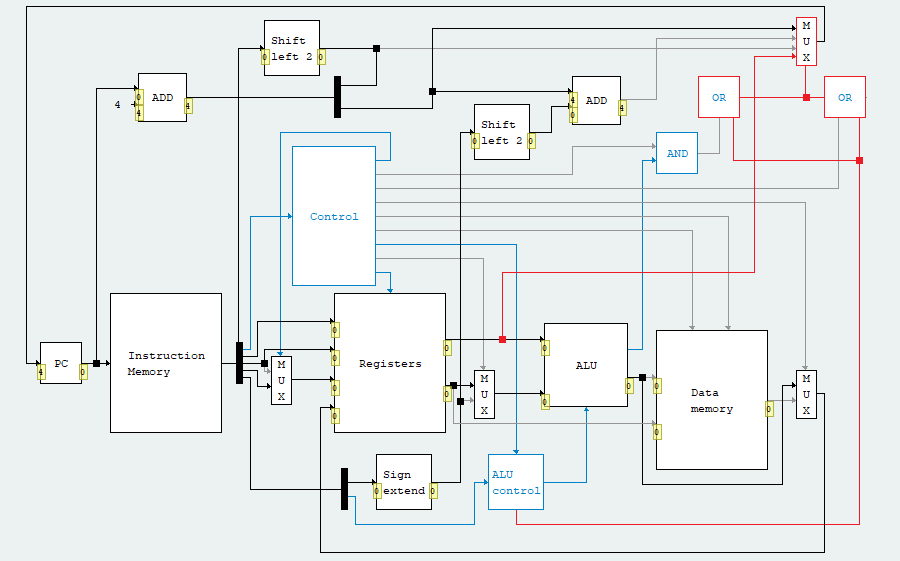
\includegraphics[scale=.7]{./img/jr_unicycle.png}
\captionof{figure}{Implementación de la instrución JR en la microarquitectura unicycle.cpu }
\label{fig:jr_unicycle}
\end{figure}

\subsection{JALR para unicycle.cpu}

La instrucción JALR (para Jump And Link Register), es casi el mismo de JR. Las únicas diferencias son que tiene func = 9 y que escribe PC+4 al registro especificado por Rd.

Añadí otra señal "link" al unidad de control del ALU, y Uso para elegir que valor a escribir al banco de registros. Figura \ref{fig:jalr_unicycle} muestra mi implementación.

Será posible solo tener una salida extra del unidad de control ALU para JR y JALR en vez de dos, si implementamos JR cómo "JALR Rs, R0".

\begin{figure}[h]
\centering
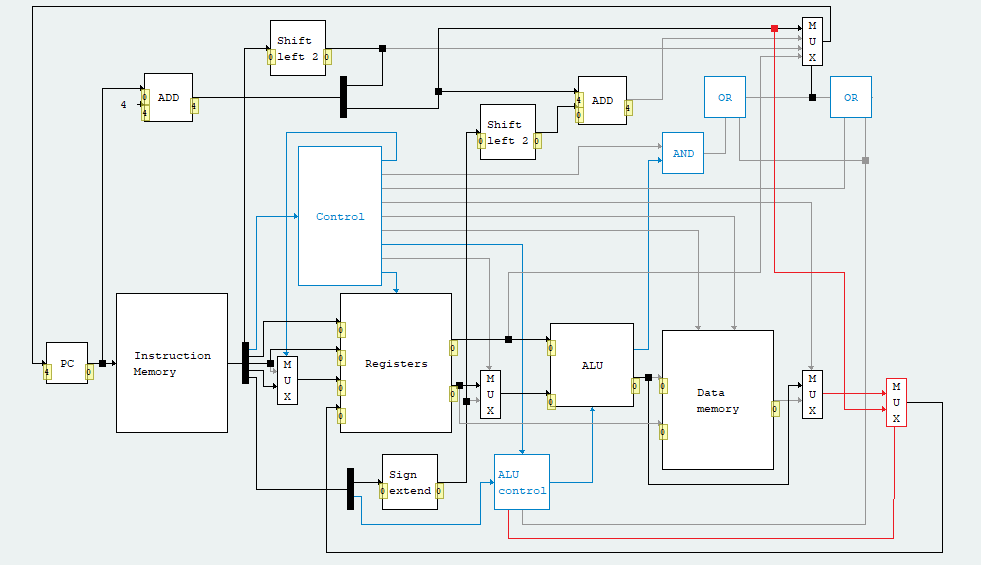
\includegraphics[scale=.6]{./img/jalr_unicycle.png}
\captionof{figure}{Implementación de la instrución JALR en la microarquitectura unicycle.cpu }
\label{fig:jalr_unicycle}
\end{figure}

\subsection{JR y JALR para pipeline.cpu}

La lógica para esas instrucciones es un poco más complicado en el CPU con un pipeline. Se ejecuta los saltos en la etapa de \textit{EX}. Sería mejor hacerles en la etapa de \textit{ID}, porque solo necesitaría un ciclo de stall en vez de dos.

Figura \ref{fig:jalr_pipeline} muestra mi implementación. De nuevo cambio el mux de nuevo PC hasta uno con cuatro entradas, y la nueva entrada toma el valor del registro especificado en Rs durante la etapa de \textit{EX}.

Tengo que flushear el registro ID/EX si hay un branch o un JR/JALR en la etapa de \textit{EX} corriente. Y tengo que flushear el registro IF/ID en el mismo caso y también si hay un salto normal en la etapa de \textit{ID}.

Hice una tabla de lógica para encontrar cómo elegir el nuevo PC. Tenemos tres señales de control:
\begin{itemize}[noitemsep]
\item J - viene de la etapa \textit{ID}.
\item JR - viene de la etapa \textit{EX}.
\item B - viene de la etapa \textit{MEM}.
\end{itemize}

Hay cuatro entradas del MUX:
\begin{itemize}[noitemsep]
\item 00 - PC+4
\item 01 - branch target
\item 10 - jump target
\item 11 - jump register
\end{itemize}

Porque las señales de control viene de etapas deferentes, unas tienen que tener preferencia sobre otras. Específicamente B viene de la instrucción más viejo, después JR, después J.

\begin{tabular}{| r r r | l r r |}
\hline
J & JR & B      & Mux                 & Mux1    & Mux0 \\ \hline
0 & 0  & 0      & 00 PC+4             & 0       & 0    \\
0 & 0  & 1      & 01 Branch Target    & 0       & 1    \\
0 & 1  & 0      & 11 Jump Register    & 1       & 1    \\
0 & 1  & 1      & 01 Branch Target    & 0       & 1    \\
1 & 0  & 0      & 10 Jump Target      & 1       & 0    \\
1 & 0  & 1      & 01 Branch Target    & 0       & 1    \\
1 & 1  & 0      & 11 Jump Register    & 1       & 1    \\
1 & 1  & 1      & 01 Branch Target    & 0       & 1    \\ \hline
\end{tabular} \\

La lógica es: Mux0 = JR o B, Mux1 = (J o JR) y !B.

Después tiene que escribir PC+4 al banco de registros en el registro especificado por Rd. Hay un riesgo de data RAW aquí, porque la siguiente instrucción puede usar el registro de destino como fuente, antes de que es escrito. Así usa \textit{forwarding} para pasar ese PC+4 a la etapa de \textit{EX}.

\begin{figure}[h]
\centering
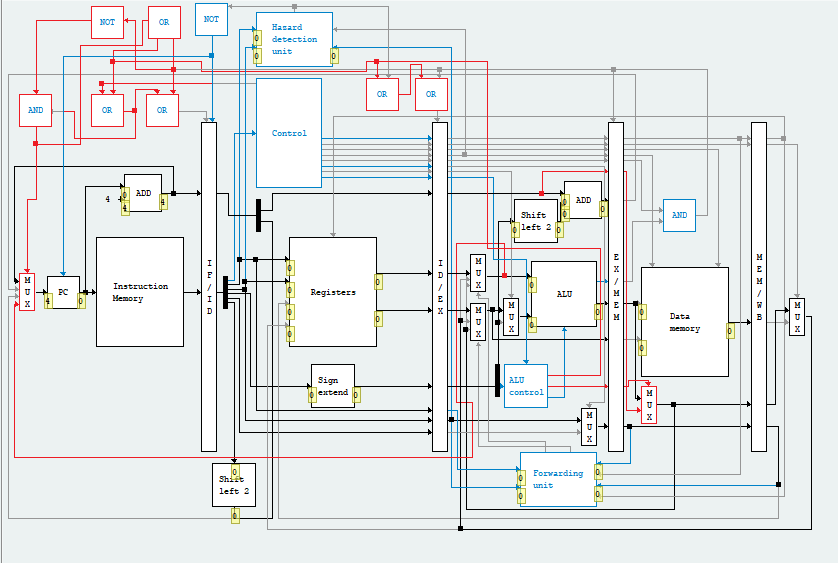
\includegraphics[scale=.7]{./img/jalr_pipeline.png}
\captionof{figure}{Implementación de la instrución JR y JALR en la microarquitectura pipeline.cpu }
\label{fig:jalr_pipeline}
\end{figure}

\section{Verificación}

Escribí una prueba para verificar el comportamiento de mis diseños. Tiene varios combinaciones de operaciones aritméticos, J, JR, JALR y branch.

\section{Archivos de diseño y pruebas}

Los archivos de diseños y prueba pueden ser encontrado en mi repositorio de github: \url{https://github.com/andrewparlane/orga6620/tree/master/tp3}.

\end{document}
